\documentclass[tikz,border=5pt]{standalone}
\usepackage{amsmath}
\usetikzlibrary{arrows.meta,positioning,calc}

\definecolor{obsfill}{HTML}{DDEBF7}
\definecolor{obsborder}{HTML}{2F5597}
\definecolor{basefill}{HTML}{EFEFEF}
\definecolor{baseborder}{HTML}{595959}
\definecolor{resfill}{HTML}{FBE5D6}
\definecolor{resborder}{HTML}{C55A11}
\definecolor{predfill}{HTML}{E2F0D9}
\definecolor{predborder}{HTML}{548235}
\definecolor{evalborder}{HTML}{404040}
\definecolor{arrowgray}{HTML}{333333}

\begin{document}
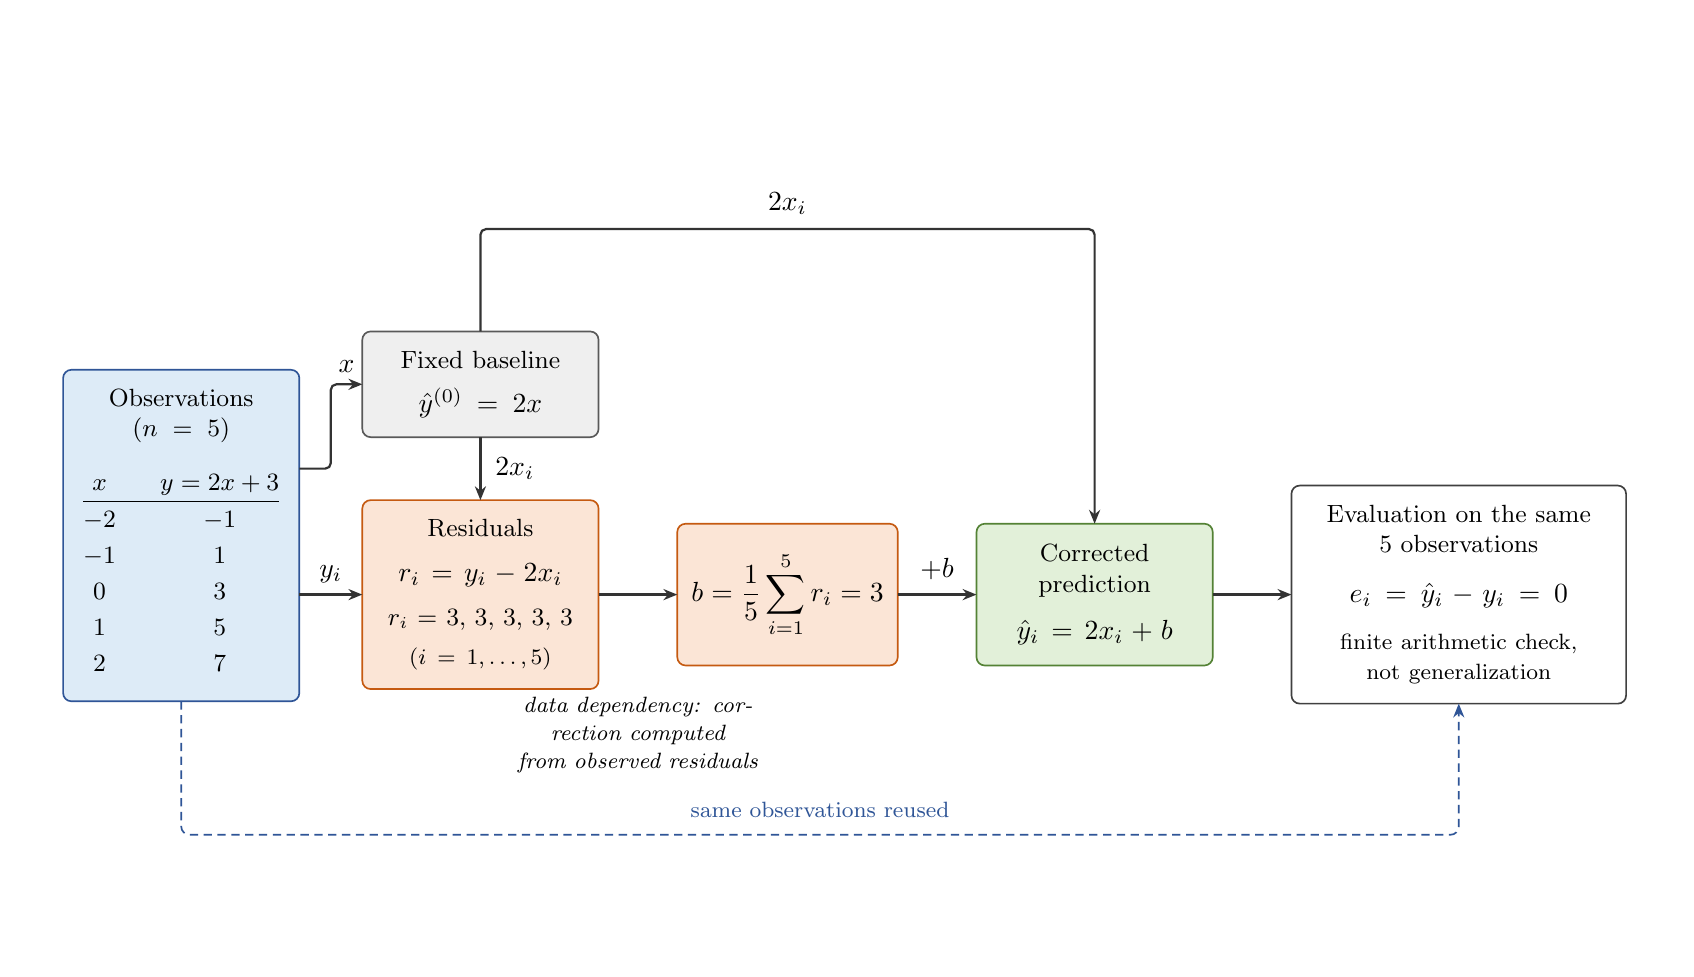
\begin{tikzpicture}[
  font=\fontsize{9}{11}\selectfont,
  box/.style={
    rectangle,
    rounded corners=3pt,
    line width=0.6pt,
    align=center,
    inner xsep=4pt,
    inner ysep=7pt,
    outer sep=0pt
  },
  observation/.style={
    box,draw=obsborder,fill=obsfill,
    minimum width=3cm,text width=2.65cm,
    minimum height=3.3cm
  },
  baseline/.style={
    box,draw=baseborder,fill=basefill,
    minimum width=3cm,text width=2.65cm,
    minimum height=1.3cm
  },
  residual/.style={
    box,draw=resborder,fill=resfill,
    minimum width=3cm,text width=2.7cm,
    minimum height=1.8cm
  },
  correction/.style={
    box,draw=resborder,fill=resfill,
    minimum width=2.8cm,text width=2.5cm,
    minimum height=1.8cm
  },
  prediction/.style={
    box,draw=predborder,fill=predfill,
    minimum width=3cm,text width=2.7cm,
    minimum height=1.8cm
  },
  evaluation/.style={
    box,draw=evalborder,fill=white,
    minimum width=4.25cm,text width=3.8cm,
    minimum height=2.3cm,
    inner xsep=6pt
  },
  computation/.style={
    draw=arrowgray,
    line width=0.8pt,
    -{Stealth[length=5pt,width=4pt]},
    rounded corners=2pt
  },
  reuse/.style={
    draw=obsborder,
    line width=0.6pt,
    dash pattern=on 3pt off 2pt,
    -{Stealth[length=5pt,width=4pt]},
    rounded corners=3pt
  },
  mathlabel/.style={
    font=\fontsize{10}{12}\selectfont,
    fill=white,
    inner sep=2pt
  }
]

% Explicit 16:9 drawing canvas. Native widths preserve readable
% typography, the evaluation text, and all requested interstage gaps.
\path[use as bounding box]
  (-0.45,-4.5) rectangle (20.35,7.2);
\fill[white] (-0.45,-4.5) rectangle (20.35,7.2);

% Stage 1: observations.
\node[observation] (obs) at (1.5,0.75) {%
  Observations ($n=5$)\\[7pt]
  \begingroup
  \renewcommand{\arraystretch}{1.18}
  \setlength{\tabcolsep}{8pt}
  \begin{tabular}{@{}cc@{}}
    $x$ & $y=2x+3$\\
    \hline
    $-2$ & $-1$\\
    $-1$ & $1$\\
    $0$  & $3$\\
    $1$  & $5$\\
    $2$  & $7$
  \end{tabular}
  \endgroup
};

% Stage 2: baseline above residual computation.
\node[residual,right=0.8cm of obs,yshift=-0.75cm] (res) {%
  Residuals\\[5pt]
  {\fontsize{10}{12}\selectfont $r_i=y_i-2x_i$}\\[5pt]
  $r_i=3,\,3,\,3,\,3,\,3$\\[3pt]
  {\fontsize{8}{10}\selectfont $(i=1,\dots,5)$}
};

\node[baseline,above=0.8cm of res] (base) {%
  Fixed baseline\\[5pt]
  {\fontsize{10}{12}\selectfont $\hat{y}^{(0)}=2x$}
};

% Stages 3--5.
\node[correction,right=1cm of res] (bias) {%
  {\fontsize{10}{12}\selectfont
    $\displaystyle b=\frac{1}{5}\sum_{i=1}^{5}r_i=3$}
};

\node[prediction,right=1cm of bias] (pred) {%
  Corrected prediction\\[6pt]
  {\fontsize{10}{12}\selectfont $\hat{y}_i=2x_i+b$}
};

\node[evaluation,right=1cm of pred] (eval) {%
  Evaluation on the same\\
  5 observations\\[7pt]
  {\fontsize{10}{12}\selectfont $e_i=\hat{y}_i-y_i=0$}\\[7pt]
  {\fontsize{8}{10}\selectfont
    finite arithmetic check,\\
    not generalization}
};

% Observed x values enter the fixed baseline through a stepped route.
\coordinate (xsource) at ($(obs.east)+(0,0.85cm)$);
\coordinate (xstep) at ($(xsource)+(0.4cm,0)$);
\draw[computation]
  (xsource) -- (xstep)
  -- (xstep |- base.west)
  -- node[mathlabel,above=2pt] {$x$} (base.west);

% Observed outcomes and baseline predictions define the residuals.
\draw[computation]
  (obs.east |- res.west)
  -- node[mathlabel,above=2pt] {$y_i$} (res.west);

\draw[computation]
  (base.south)
  -- node[mathlabel,right=3pt] {$2x_i$} (res.north);

% Residuals determine the scalar correction.
\draw[computation] (res.east) -- (bias.west);
\coordinate (dependencymid) at ($(res.east)!0.5!(bias.west)$);

\node[
  anchor=north,
  align=center,
  text width=4.2cm,
  inner sep=0pt,
  font=\fontsize{8}{10}\selectfont\itshape
] at ($(dependencymid)+(0,-1.3cm)$) {%
  data dependency: correction computed\\
  from observed residuals
};

% The baseline contribution follows a separate upper corridor.
\coordinate (basetop) at ($(base.north)+(0,1.3cm)$);
\draw[computation]
  (base.north) -- (basetop)
  -- node[mathlabel,above=3pt] {$2x_i$}
     (basetop -| pred.north)
  -- (pred.north);

\draw[computation]
  (bias.east)
  -- node[mathlabel,above=3pt] {$+b$} (pred.west);

\draw[computation] (pred.east) -- (eval.west);

% A dedicated lower corridor makes reuse of the observations explicit.
\coordinate (reuseleft) at (obs.south |- 0,-3.05);
\coordinate (reuseright) at (eval.south |- 0,-3.05);
\draw[reuse]
  (obs.south) -- (reuseleft)
  -- node[
    midway,
    above=4pt,
    text=obsborder,
    fill=white,
    inner sep=2pt,
    font=\fontsize{8}{10}\selectfont
  ] {same observations reused}
  (reuseright) -- (eval.south);

\end{tikzpicture}
\end{document}